\documentclass[journel,12pt,twocoloums]{IEEEtran}

\title{Assignment 9-Probability and Random Variable}
\author{Annu-EE21RESCH01010}
\date{13 January 2020}

\usepackage{amsthm}
\usepackage{graphicx}
\usepackage{mathrsfs}
\usepackage{txfonts}
\usepackage{stfloats}
\usepackage{pgfplots}
\usepackage{cite}
\usepackage{cases}
\usepackage{mathtools}
\usepackage{caption}
\usepackage{enumerate}	
\usepackage{enumitem}
\usepackage{amsmath}
\usepackage[utf8]{inputenc}
\usepackage[english]{babel}
\usepackage{multicol}
%\usepackage{xtab}
\usepackage{longtable}
\usepackage{multirow}
%\usepackage{algorithm}
%\usepackage{algpseudocode}
\usepackage{array,multirow}
\usepackage{enumitem}
\usepackage{mathtools}
\usepackage{gensymb}
\usepackage{hyperref}
%\usepackage[framemethod=tikz]{mdframed}
\usepackage{listings}
    %\usepackage[latin1]{inputenc}                                 %%
    \usepackage{color}                                            %%
    \usepackage{array}                                            %%
    \usepackage{longtable}                                        %%
    \usepackage{calc}                                             %%
    \usepackage{multirow}                                         %%
    \usepackage{hhline}                                           %%
    \usepackage{ifthen}                                         %%
  \providecommand{\nCr}[2]{\,^{#1}C_{#2}}
  \providecommand{\nPr}[2]{\,^{#1}P_{#2}}
  \lstset{
%language=C,
frame=single, 
breaklines=true,
columns=fullflexible
}

 \begin{document}
 \maketitle
\textbf{Download latex code from here-}\\
\begin{lstlisting}
 https://github.com/annu100/AI5002-Probability-and-Random-variables/tree/main.tex/ASSIGNMENT_9
 \end{lstlisting}
 \textbf{Download python code from here-}\\
\begin{lstlisting}
 https://github.com/annu100/AI5002-Probability-and-Random-variables/tree/main.py/ASSIGNMENT_9
 \end{lstlisting}
 \section{Problem Statement-Problem 5.24}

One card is drawn from a well-shuffled deck
of 52 cards. Calculate the probability that the
card will
(i) be an ace,
(ii) not be an ace.
Simulation part -
Represent the given problem in terms of bernoulli random variables and plot it's associated distributions.
\section{SOLUTIONS}
let A be the event of getting an ace card.
In a dec of 52 cards,4 ace cards are there in total.
so,probability for getting an ace card is given by,
therefore,
P(A) =$\frac{4}{52}$=$\frac{1}{13}$\\
Therefore,probability for getting ace card is $\frac{1}{13}$.\\
\\
\\
let B be the event of not getting an ace card.\\
P(B) =1-P(A)=1-$\frac{1}{13}$=$\frac{12}{13}$\\
Therefore,probability for not getting ace card is $\frac{12}{13}$.



\subsection{Bernaulli random variables simulation}

\begin{figure}[!ht]

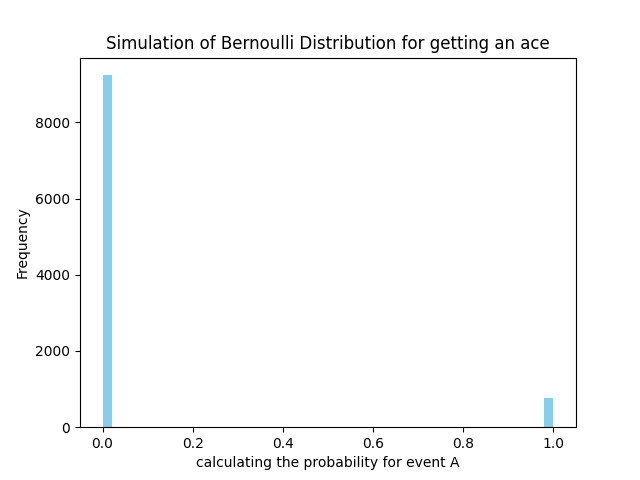
\includegraphics[width=\columnwidth] {Figure_1.png}
\caption{For random variable A}

\end{figure}
\\

 \begin{figure}

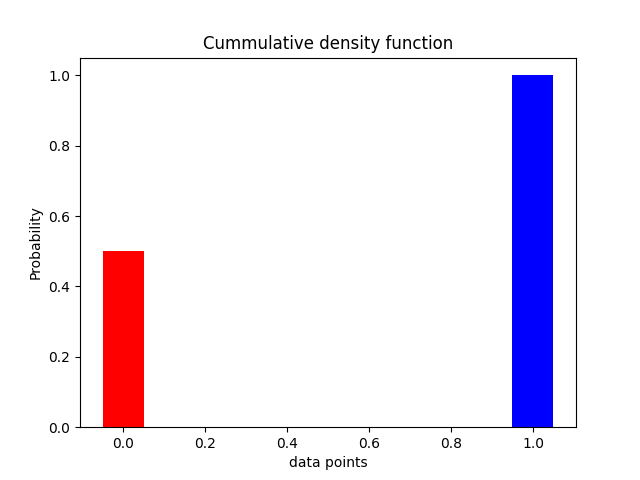
\includegraphics[width=\columnwidth] {Figure_2.png}
\caption{For random variable B}

\end{figure}

\end{document}

        

